\documentclass[spec, och, otchet, hidelinks]{SCWorks}
% параметр - тип обучения - одно из значений:
%    spec     - специальность
%    bachelor - бакалавриат (по умолчанию)
%    master   - магистратура
% параметр - форма обучения - одно из значений:
%    och   - очное (по умолчанию)
%    zaoch - заочное
% параметр - тип работы - одно из значений:
%    otchet
%    referat    - реферат
%    coursework - курсовая работа (по умолчанию)
%    diploma    - дипломная работа
%    pract      - отчет по практике
%    pract      - отчет о научно-исследовательской работе
%    autoref    - автореферат выпускной работы
%    assignment - задание на выпускную квалификационную работу
%    review     - отзыв руководителя
%    critique   - рецензия на выпускную работу
% параметр - включение шрифта
%    times    - включение шрифта Times New Roman (если установлен)
%               по умолчанию выключен
\usepackage[T2A]{fontenc}
\usepackage[utf8]{inputenc}
\usepackage{graphicx}

\usepackage[sort,compress]{cite}
\usepackage{amsmath}
\usepackage{amssymb}
\usepackage{amsthm}
\usepackage{fancyvrb}
\usepackage{longtable}
\usepackage{array}
\usepackage[english,russian]{babel}
\usepackage{listings}
\usepackage{xcolor}
% Используется автором репозитория
%\usemintedstyle{xcode}
% Этот пакет включает в себя аналогичный Times New Roman шрифт.
% Необходим для успешной компиляции для UNIX-систем ввиду отсутствия TNR в нем.
% Можно использовать и для Windows.
\usepackage{tempora}

\lstset{%
	language=C,
	backgroundcolor=\color{gray!12},
	basicstyle=\ttfamily\small,
	keywordstyle=\color{blue},
	stringstyle=\color{blue},
	showstringspaces=false,
	captionpos=b,
	numbers=left,
	numberstyle=\footnotesize\color{gray},
	frame=TB,
	tabsize=2,
	morekeywords={procedure, then, begin, end}
}

\usepackage[colorlinks=false]{hyperref}

\graphicspath{{figures/}}

\newcommand{\eqdef}{\stackrel {\rm def}{=}}

\usepackage{stackengine}
\newcommand\xrowht[2][0]{\addstackgap[.5\dimexpr#2\relax]{\vphantom{#1}}}
\newcommand{\tbf}[1]{\textbf{#1}}
\newtheorem{lem}{Лемма}

% % При использовании biblatex вместо bibtex
%\usepackage[style=gost-numeric]{biblatex}
%\addbibresource{thesis.bib}

\begin{document}

% Кафедра (в родительном падеже)
\chair{математической кибернетики и компьютерных наук}

% Тема работы
\title{Преобразователи кодов}

% Курс
\course{3}

% Группа
\group{331}

% Факультет (в родительном падеже) (по умолчанию "факультета КНиИТ")
%\department{факультета КНиИТ}

% Специальность/направление код - наименование
%\napravlenie{02.03.02 "--- Фундаментальная информатика и информационные технологии}
%\napravlenie{02.03.01 "--- Математическое обеспечение и администрирование информационных систем}
%\napravlenie{09.03.01 "--- Информатика и вычислительная техника}
%\napravlenie{09.03.04 "--- Программная инженерия}
\napravlenie{10.05.01 "--- Компьютерная безопасность}

% Для студентки. Для работы студента следующая команда не нужна.
%\studenttitle{Студентки}

% Фамилия, имя, отчество в родительном падеже
\author{Бородина Артёма Горовича}

% Заведующий кафедрой
\chtitle{доцент, к.\,ф.-м.\,н.} % степень, звание
\chname{С.\,В.\,Миронов}

%Научный руководитель (для реферата преподаватель проверяющий работу)
\satitle{аспирант}%, к.\,ф.-м.\,н.} %должность, степень, звание
\saname{А.\,А.\,Мартышкин}

% Руководитель практики от организации (только для практики,
% для остальных типов работ не используется)
\patitle{к.\,ф.-м.\,н., доцент}
\paname{Д.\,Ю.\,Петров}

% Семестр (только для практики, для остальных
% типов работ не используется)
\term{2}

% Наименование практики (только для практики, для остальных
% типов работ не используется)
\practtype{учебная}

% Продолжительность практики (количество недель) (только для практики,
% для остальных типов работ не используется)
\duration{2}

% Даты начала и окончания практики (только для практики, для остальных
% типов работ не используется)
\practStart{01.07.2016}
\practFinish{14.07.2016}

% Год выполнения отчета
\date{2022}

\maketitle

% Включение нумерации рисунков, формул и таблиц по разделам
% (по умолчанию - нумерация сквозная)
% (допускается оба вида нумерации)
%\secNumbering


\tableofcontents

% Раздел "Обозначения и сокращения". Может отсутствовать в работе
% \abbreviations
% \begin{description}
%     \item ... "--- ...
%     \item ... "--- ...
% \end{description}

% Раздел "Определения". Может отсутствовать в работе
%\definitions

% Раздел "Определения, обозначения и сокращения". Может отсутствовать в работе.
% Если присутствует, то заменяет собой разделы "Обозначения и сокращения" и "Определения"
%\defabbr


% Раздел "Введение"

\section{Цель работы и порядок выполнения}

Цель работы — изучение основных понятий теории полугрупп. \\

\par \textbf{Порядок выполнения работы}
\begin{enumerate}
\item Рассмотреть понятия полугруппы, подполугруппы и порождающего множества.
  Разработать алгоритм построения подполугрупп по таблице Кэли.
\item Разработать алгоритм построения полугруппы бинарных отношений по заданному
  порождающему множеству.
\item Рассмотреть понятия подгруппы, порождающего множества и определяющих
  соотношений. Разработать алгоритм построения полугруппы по порождающему
  множеству и определяющим соотношениям.
\end{enumerate}
  
\newpage

\section{Теоретические сведения по рассмотренным темам с их обоснованием}

\par \tbf{Определение}. $\,$ \textit{Полугруппа} – это алгебра $S = (S, \cdot)$ с одной
ассоциативной бинарной операцией $\cdot$, т.е. выполняется $(x \cdot y) \cdot z
= x \cdot (y \cdot z) $ для любых $x, y, z \in S.$ Если полугрупповая операция называется умножением
(соответственно, сложением), то полугруппу называют \textit{мультипликативной}
(соответственно, \textit{аддитивной}).

\par \tbf{Определение}. Подмножество $X$ полугруппы $S$ называется
\textit{подполугруппой}, если $X$ устойчиво относительно операции
умножения, т.е. для любых $x, y \in X$ выполняется свойство: $x \cdot y \in X$.
В этом случае множество X с ограничением на нем операции
умножения исходной полугруппы S образует полугруппу. \\

\par \tbf{Определение} (\textit{Порождающее множество}). В силу общего свойства
подалгебр пересечение любого семейства $X_i$
$(i\in I)$ подполугрупп полугруппы $S$ является подполугруппой $S$ и,
значит, множество $Sub(S)$ всех подполугрупп полугруппы $S$ является
системой замыканий. Следовательно, для любого подмножества $X$
полугруппы $S$ существует наименьшая подполугруппа $S$, содержащая
множество $X$. Такая полугруппа обозначается символом <$X$> и
называется подполугруппой $S$, порождённой множеством $X$. При
этом множество $X$ называется также порождающим множеством
подполугруппы <$X$>. 

\par В частности, если <$X$> = $S$, то $X$ называется \textit{порождающим
множеством полугруппы} $S$ и говорят, что множество $X$ порождает
полугруппу $S$. 

\par Видно, что полугруппа <$X$> состоит из всевозможных
конечных произведений $x_1 \cdot ... \cdot x_n$ элементов $x_1, \dots, x_n \in
X$, т.е. выполняется равенство: $$ 〈X〉 = \{x_1 \cdot ... \cdot x_n: n \in N \;
\text{и} \; x_1, \dots, x_n \in X\} $$

\par \tbf{Алгоритм вычисления подполугруппы $〈X〉 \subset S:$}
\begin{enumerate}
\item Положим $i = 0, \; X_0 = X$.
\item Для $X_i$ вычислим $\overline X_l = \{x \cdot y : x \in X_i \wedge y \in
  X\}$ и положим $X_{i + 1} = X_i \cup \overline X_l$.
\item Вычисляем $〈X〉 = \bigcup\limits_{i = 0}^{\infty} X_i$.
\end{enumerate}

\newpage

\par \tbf{Определение} (\textit{Определяющее соотношение и копредставление
  полугруппы S}). Для любой конечной
полугруппы $S$ найдется такой конечный алфавит $A$, что для некоторого отображения
$ \varphi: A \rightarrow S$ выполняется равенство <$\varphi(A)$> = $S$ и,
значит, $S \cong A^{+} \slash \ker \varphi$. В это случае множество $A$
называется \textit{множеством порождающих символов} полугруппы $S$ (относительно
отображения $\varphi: A \rightarrow S $). Если при этом для слов $w_1, w_2 \in
A^{+}$ выполняется равенство $\varphi(w_1) = \varphi(w_2)$, т.е. $w_1 \equiv w_2
(\ker \varphi)$, то говорят, что на $S$ \textit{выполняется соотношение} $w_1 =
w_2$ (относительно отображения $\varphi: A \rightarrow S$).

\par В некоторых случаях можно выбрать подмножество $\rho \subset \ker \varphi$,
которое однозначно определяет конгруэнцию $\ker \varphi$ как наименьшую
конгруэнцию полугруппы $A^{+}$, содержащую отношение $\rho$, т.е. $\ker \varphi
= f_{con}(\rho) = f_{eq}(f_{reg}(\rho))$. В случае $(w_1, w_2) \in \rho$ будет
выполняться равенство $\varphi (w_1) = \varphi (w_2)$ -- будем называть такие
выражения \textit{определяющими соотношениями}. Из таких соотношений конгруэнция
$\ker \varphi$ строится с помощью применения следующих процедур к словам $u, v
\in A^{+}$:
\begin{enumerate}
\item слово $v$ \textit{непосредственно выводится} из слова $u$, если $v$
  получается из $u$ заменой некоторого подслова $w_1$ на слово $w_2$,
  удовлетворяющее определяющему соотношению $w_1 = w_2$, т.е. $(u, v) =
  (xw_1y, xw_2y)$ для некоторых $x, y \in A^{*}$;
\item слово $v$ \textit{выводится} из слова $u$, если $v$ получается из $u$ с
  помощью конечного числа применения процедуры (1).
\end{enumerate}

\par Если все выполняющиеся на $S$ соотношения выводятся из определяющих
соотношений совокупности $\rho$, то конгруэнция $\ker \varphi$ полностью
определяется отношением $\rho$ и выражение $$ <A : \{w_1 = w_2 : (w_1, w_2) \in
\rho\}> $$ называется \textit{копредставлением полугруппы S}.
  
\newpage

\section{Результаты работы}

\subsection{Алгоритм построения подполугруппы по заданному порождающему множеству}
\par \tbf{Описание алгоритма построения подполугруппы по заданному порождающему
  множеству.} \\
\tbf{Вход:} полугруппа $S$ с таблицей Кэли размерности $N \times N$, а также порождающее
множество $X \subset S$. \\
\tbf{Выход:} построенная подполугруппа <$X$> $\subset S$. \\
\tbf{Метод:} вычисляем подполугруппу <$X$> в соответствии с упомянутым
алгоритмом. На каждом шаге новые элементы добавляем в структуру $set$,
содержащую только уникальные элементы. Если после вычисления $\overline X_l$, а
затем $X_{i + 1} = X_i \cup \overline X_l$ ($X_{i}$ определяется структурой
$set$) размер контейнера не увеличился, это означает, что в него не было
добавлено новых элементов, что в свою очередь свидетельствует о том, что процесс
вычисления подполугруппы <$X$> $\subset S$ закончен.

\par \tbf{Псевдокод алгоритма построения подполугруппы по заданному порождающему
множеству.}
\begin{lstlisting}[caption=Псевдокод алгоритма., mathescape]
get_subsemigroup(<N$\times$N matrix> CayleyTable, semigroupSubset[])
{
  <set> newElements, $X_i$ = semigroupSubset;
  while (true)
  {
    currentSize = $X_i$.size();
    for object in $X_i$:
      for diffObject in $X_i$:
        newElements.insert(
          CayleyTable[row_in_table(object)]
                     [col_in_table(diffObject)]);
    for newItem in newElements:
      $X_i$.insert(newItem);
    if ($X_i$.size() == currentSize)
      break;
    newElements.clear();
  }
  return $X_i$;
}
\end{lstlisting}

\par \tbf{Код программы построения подполугруппы по заданному порождающему множеству.}
\begin{lstlisting}[caption=Код программы., mathescape]
void getSubsemigroupMachinerie (vector<vector<int>> CayleyTable, 
                                set<int>& subsemigroup)
{
  set<int> ::iterator i, j;
  set<int> newElements, X_i = semigroupSubset;

  while (true)
    {
      unsigned short curSize = X_i.size ();

      for (i = X_i.begin (); i != X_i.end (); ++i)
        for (j = X_i.begin (); j != X_i.end (); ++j)
          newElements.insert (CayleyTable[*i][*j]);
      for (i = newElements.begin(); i != newElements.end(); ++i)
        X_i.insert (*i);
      if (X_i.size () - curSize == 0)
        break;
      newElements.clear ();
    }
  subsemigroup = X_i;
}
\end{lstlisting}

\newpage

\par \tbf{Результат тестирования программы построения подполугруппы по заданному
порождающему множеству.}

\par Рассмотрим полугруппу $S = \{a, b, c, d\}$ с таблицей Кэли размерности 4
$\times$ 4 и порождающим множеством $X$ $\subset S = \{b\}$. Построим
подполугруппу <$X$> $\subset S$ по заданным входным данным.

\begin{figure}[h!]
  \center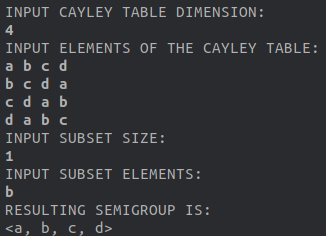
\includegraphics[scale=0.65]{construct_semigroup.png}
  \caption{Результат построения подполугруппы <$X$> по заданному порождающему
    множеству.}
\end{figure}

\par Получилось, что <$X$> = $S$, и $X = \{b\}$ является \textit{порождающим множеством
  полугруппы S}. \\

\par \tbf{Оценка сложности алгоритма построения подполугруппы по заданному
  порождающему множеству.}
\par Для генерации новых элементов ищутся все попарные произведения элементов из
контейнера $X_i$. Значения этих произведений хранятся в заданной таблице Кэли.
Количество элементов в $X_i$ на каждом шаге не превышает размера заданной
полугруппы $S$, т.е. числа строк или столбцов в заданной таблице Кэли ($N$). Внешний
цикл $while$ сработает не более $N$ раз, т.к. алгоритм будет работать, пока на
каждом шаге в $X_i$ будет добавляться один или более элемент. Таким образом,
оценка сложности алгоритма построения подполугруппы по заданному порождающему
множеству принимает вид: $O(N^3)$.

\newpage

\subsection{Алгоритм построения полугруппы бинарных отношений по заданному
  порождающему множеству}
\par \tbf{Описание алгоритма построения полугруппы бинарных отношений по
  заданному порождающему множеству.} \\
\tbf{Вход:} порождающее множество $X$ матриц бинарных отношений. \\
\tbf{Выход:} полугруппа <$X$> и таблица Кэли полученной полугруппы. \\
\tbf{Метод:} аналогичен методу построения подполугруппы по заданному
порождающему множеству. Если на некотором шаге после вычисления попарных композиций бинарных
отношений не было сформировано новых элементов, то процесс построения полугруппы
окончен, и программа переходит к построению таблицы Кэли полученной полугруппы.

\par \tbf{Псевдокод алгоритма построения полугруппы бинарных отношений по
  заданному порождающему множеству.}
\begin{lstlisting}[caption=Псевдокод алгоритма., mathescape]
get_semigroup(<set <N$\times$N matrix>> binaryRelationSet)
{
  <set <N$\times$N matrix>> newElements, $X_i$ = binaryRelationSet;
  while (true)
  {
    currentSize = $X_i$.size();
    for binRelMat in $X_i$:
      for diffBinRelMat in $X_i$:
        newElements.insert(
          get_binary_relation_composition(
            binRelMat, diffBinRelMat);
    for newItem in newElements:
      $X_i$.insert(newItem);
    if ($X_i$.size() == currentSize)
      break;
    newElements.clear();
  }
  return $X_i$;
}
\end{lstlisting}

\newpage

\par \tbf{Код программы построения полугруппы бинарных отношений по заданному
  порождающему множеству.}
\begin{lstlisting}[caption=Код программы., mathescape]
vector<vector<unsigned short>> boolMatricesMultiplication (
  vector<vector<unsigned short>> fM, 
  vector<vector<unsigned short>> sM)
{
  unsigned short i, j, k, matSize = fM.size (), product = 0;
  vector<vector<unsigned short>> resM (
    matSize, vector<unsigned short> (matSize, 0));

  for (i = 0; i < matSize; ++i)
    for (j = 0; j < matSize; ++j)
      {
        for (k = 0; k < matSize; ++k)
          product += fM[i][k] * sM[k][j];
        resM[i][j] = (product > 0 ? 1 : 0);
        product = 0;
      }
  return (resM);
}

vector<pair<vector<vector<unsigned short>>, char>> 
  matrixMappings;
char symbolToMap = 'a';

void getSemigroupMachinerie (
  set<vector<vector<unsigned short>>> binaryRelationSet, 
  set<vector<vector<unsigned short>>>& semigroup)
{
  set<vector<vector<unsigned short>>> ::iterator i, j;
  set<vector<vector<unsigned short>>> newElements, 
                                      X_i = binaryRelationSet;

  while (true)
    {
      unsigned short curSize = X_i.size ();

      for (i = X_i.begin (); i != X_i.end (); ++i)
        for (j = X_i.begin (); j != X_i.end (); ++j)
          newElements.insert (
            boolMatricesMultiplication (*i, *j));
      for (i = newElements.begin(); i != newElements.end(); ++i)
        X_i.insert (*i);
      if (X_i.size () - curSize == 0)
        break;
      newElements.clear ();
    }
  semigroup = X_i;
}

char find_corresponding_letter (
  vector<pair<vector<vector<unsigned short>>, char>> matMaps, 
  vector<vector<unsigned short>> matToCheck)
{
  int i;
  for (i = 0; i < matMaps.size (); ++i)
    if (matMaps[i].first == matToCheck)
      return (matMaps[i].second);
  return ('.');
}

void display_matrix_Cayley_table (
  vector<pair<vector<vector<unsigned short>>, char>> matMaps)
{
  int i, j;

  cout << endl << "CAYLEY TABLE:\n";
  cout << "    ";
  for (i = 0; i < matMaps.size (); ++i)
    cout << setw (4) << matMaps[i].second;
  cout << "\n";

  for (i = 0; i < matMaps.size (); ++i)
    {
      cout << setw (4) << matMaps[i].second << setw (4);
      for (j = 0; j < matMaps.size (); ++j)
        cout << find_corresponding_letter (
          matMaps, 
          boolMatricesMultiplication (matMaps[i].first, 
                                      matMaps[j].first)) 
           << setw (4);
      cout << "\n";
    }
  cout << endl;
}

void getSemigroup ()
{
  unsigned short i = 0, j, k = 0, binaryRelationsNumber;
  set<vector<vector<unsigned short>>> ::iterator it;
  set<vector<vector<unsigned short>>> binaryRelationSet, 
                                      semigroup;
  cout << "INPUT THE NUMBER OF BINARY RELATIONS:\n";
  cin >> binaryRelationsNumber;
  cout << "INPUT THE DIMENSION OF MATRICES:\n";
  cin >> matrixDimension;

  while (i < binaryRelationsNumber)
    {
      vector<vector<unsigned short>> 
        binaryRelationMatrix (
          matrixDimension, vector<unsigned short> (
                             matrixDimension, 0));
      cout << "INPUT THE BINARY RELATION MATRIX:\n";
      getMatrix (binaryRelationMatrix);

      if (binaryRelationSet.empty ())
        {
          binaryRelationSet.insert (binaryRelationMatrix);
          ++i;
          continue;
        }
      for (it = binaryRelationSet.begin (); 
           it != binaryRelationSet.end (); ++it)
        if (*it == binaryRelationMatrix)
          cout << "THIS MATRIX IS ALREADY IN THE SET. 
                   TRY ANOTHER ONE.\n";
        else
          {
            binaryRelationSet.insert (binaryRelationMatrix);
            ++i;
          }
    }
  getSemigroupMachinerie (binaryRelationSet, semigroup);

  cout << "THE RESULTING SEMIGROUP IS:\n";

  for (it = semigroup.begin (); it != semigroup.end (); ++it)
    {
      cout << symbolToMap << ":\n";
      matrixMappings.push_back (make_pair (*it, symbolToMap++));
      for (i = 0; i < matrixDimension; ++i)
        {
          for (j = 0; j < matrixDimension; ++j)
            cout << (*it)[i][j] << " ";
          cout << '\n';
        }
      cout << '\n';
    }
  display_matrix_Cayley_table (matrixMappings);
}
\end{lstlisting}
\conclusion

\end{document}